% LuaLaTeX文書; 文字コードはUTF-8
\documentclass[unicode,12pt]{beamer}% 'unicode'が必要
\usepackage{luatexja}% 日本語したい
\usepackage[ipaex]{luatexja-preset}% IPAexフォントしたい
\renewcommand{\kanjifamilydefault}{\gtdefault}% 既定をゴシック体に

\usepackage{amssymb,amsmath,ascmac}

\usepackage{multirow}
\usepackage{bm}

\graphicspath{{../fig/}}

\usepackage{tikz}
\usepackage{xparse}
\usetikzlibrary{shapes,arrows}
%% define fancy arrow. \tikzfancyarrow[<option>]{<text>}. ex: \tikzfancyarrow[fill=red!5]{hoge}
\tikzset{arrowstyle/.style n args={2}{inner ysep=0.1ex, inner xsep=0.5em, minimum height=2em, draw=#2, fill=black!20, font=\sffamily\bfseries, single arrow, single arrow head extend=0.4em, #1,}}
\NewDocumentCommand{\tikzfancyarrow}{O{fill=black!20} O{none}  m}{
\tikz[baseline=-0.5ex]\node [arrowstyle={#1}{#2}] {#3 \mathstrut};}

%目次スライド
\AtBeginSection[]{
  \frame{\tableofcontents[currentsection]}
}
%アペンディックスのページ番号除去
\newcommand{\backupbegin}{
\newcounter{framenumberappendix}
\setcounter{framenumberappendix}{\value{framenumber}}
}
\newcommand{\backupend}{
\addtocounter{framenumberappendix}{-\value{framenumber}}
\addtocounter{framenumber}{\value{framenumberappendix}} 
}

%%%%%%%%%%%  theme  %%%%%%%%%%%
\usetheme{Copenhagen}
% \usetheme{Metropolis}
% \usetheme{CambridgeUS}
% \usetheme{Berlin}

%%%%%%%%%%%  inner theme  %%%%%%%%%%%
% \useinnertheme{default}

% %%%%%%%%%%%  outer theme  %%%%%%%%%%%
\useoutertheme{default}
% \useoutertheme{infolines}

%%%%%%%%%%%  color theme  %%%%%%%%%%%
%\usecolortheme{structure}

%%%%%%%%%%%  font theme  %%%%%%%%%%%
\usefonttheme{professionalfonts}
%\usefonttheme{default}

%%%%%%%%%%%  degree of transparency  %%%%%%%%%%%
%\setbeamercovered{transparent=30}

% \setbeamertemplate{items}[default]

%%%%%%%%%%%  numbering  %%%%%%%%%%%
% \setbeamertemplate{numbered}
\setbeamertemplate{navigation symbols}{}
\setbeamertemplate{footline}[frame number]


\title{粘着技術とタッキファイヤーの基礎\\と応用展開}
\subtitle{~ 第二章 粘着剤の基礎 ~}
\author[東亞合成 佐々木]{佐々木 裕\thanks{hiroshi\_sasaki@mail.toagosei.co.jp}}
\institute[東亞合成]{東亞合成株式会社}
\date{2024/2/15}

\begin{document}

%%%%%
% 1 P
%%%%%
\maketitle

\begin{frame} 
    \tableofcontents[]
\end{frame} 


\section{粘着とは?}
\subsection{粘着と接着を比べると?}
\begin{frame}
	\frametitle{粘着と接着}
		\begin{block}{化学辞典での定義}
			\begin{itemize}
				\item 流動性の物質が被着体に接触付着することで、同種または異種の物体を貼り合わせる場合に、永久的に接着する場合と\textcolor{blue}{一時的に接着する場合があり、後者を粘着という}。
				\item 接着では、被着体に接触する際に、流動性をもたせるため、溶解、加熱などの手段を必要とするが、\textcolor{red}{粘着は、粘着物質そのものがもともと液体的性質をもっている点が異なる}。
				\item 粘着後、これを引き離そうとするときは、外力に対して\textcolor{red}{粘弾性的抵抗を示す}。
			\end{itemize}
		\end{block}
\end{frame}

\begin{frame}
	\frametitle{粘着と接着の比較}
		時間と接着強度の関係を図示すると、以下のような\\イメージになります。

		\vspace{5mm}
			\centering
				\includegraphics[width=.8\textwidth]{../fig/adh_psa.png}
		
\end{frame}

\subsection{粘着の特徴}
\begin{frame}
	\frametitle{粘着の特徴}
	\vspace{-2mm}
	\begin{block}{機能と性質}
		\begin{itemize}
			\item どちらも、物と物をくっつける(固定する)機能は同じ
			\begin{itemize}
				\item 硬化に時間が必要で剥がれてはいけないのが接着
				\item \textcolor{red}{少しの圧力でくっついて剥がすことができる}のが粘着
			\end{itemize}
			\item 性質で考えると
			\begin{itemize}
				\item 接着剤は「使う前は液体で、貼り付けると固体になる」
				\item 粘着剤は「\textcolor{red}{液体と固体の両方の性質を持ち}、常に濡れた状態を安定して保っている」
			\end{itemize}
		\end{itemize}
	\end{block}
	\vspace{-2mm}
	\begin{alertblock}{感圧接着剤: Pressure Sensitive Adhesives (PSA)}
		\begin{itemize}
			\item 常温で短時間わずかな圧力を加えただけでくっつく
			\item 剥がそうと思えば剥がすことができ
			\item 剥がすときにある程度の力が必要
		\end{itemize}
	\end{alertblock}
\end{frame}

\subsection{粘着技術の応用}
\begin{frame}
	\frametitle{粘着技術の応用}
			\begin{columns}[onlytextwidth]
				\column{.48\linewidth}
					\begin{itemize}
						\item 粘着テープへの応用
						\item 基材に粘着剤を塗布
						\begin{itemize}
							\item 一般的なテープ
							\item 両面テープ
						\end{itemize}
					\end{itemize}
				\column{.48\linewidth}
				\vspace{2mm}
				\centering
				\includegraphics[width=.8\textwidth]{nentyaku_tape.jpg}

				\vspace{-3mm}
				\href{https://tape-omakase-navi.com/column/post-14/}{\textcolor{red}{\underline{\scriptsize{この画像のサイトへのリンク}}}}
			\end{columns}
		\begin{block}{用途}
			\begin{columns}[c, onlytextwidth]
				\column{.48\linewidth}
				\centering
				\includegraphics[width=\textwidth]{car_psa.jpg}

				\vspace{-2mm}
				\href{https://www.lintec.co.jp/dream/tsunagu/products/03/}{\textcolor{red}{\underline{\scriptsize{この画像のサイトへのリンク}}}}

				\column{.48\linewidth}
				\centering
				\includegraphics[width=\textwidth]{touchpanel.png}

				\vspace{-2mm}
				\href{https://www.ojiholdings.co.jp/r_d/theme/hffilm.html}{\textcolor{red}{\underline{\scriptsize{この画像のサイトへのリンク}}}}
			\end{columns}
		\end{block}
\end{frame}

\section{なぜ、引っ付いて剥がすことができるのか?}

\subsection{引っ付くということ}
\begin{frame}
	\frametitle{引っ付くということ}
	
	\begin{block}{引っ付いている原因について}
		\begin{columns}[c, onlytextwidth]
			\column{.48\linewidth}
			これまでに多様な説が提案
				\begin{itemize}
					\item 機械的結合説
					\item 化学結合説
					\item 分子間力説
					\item 静電気説
					\item 高分子の相互貫入
					\item 等々
				\end{itemize}
			\column{.48\linewidth}
			\centering
			\includegraphics[width=.85\textwidth]{Adhesion_Overview.png}

			\vspace{-2mm}
				\href{https://www.stevenabbott.co.uk/practical-adhesion/}{\textcolor{red}{\underline{\scriptsize{この画像のサイトへのリンク}}}}
		\end{columns}
	\end{block}
\end{frame}

\begin{frame}
	\frametitle{水による接着}
		\begin{block}{水だけで二枚のガラスを引っ付ける実験}
			\begin{columns}[c, onlytextwidth]
				\column{.48\linewidth}
					\begin{itemize}
						\item 実験に使用するもの
					\end{itemize}
	
					\centering
					\includegraphics[width=.9\textwidth]{glass_water3.jpg}
	
				\column{.48\linewidth}
	
				\begin{itemize}
					\item 圧着するだけで
					\item 強く引っ付いて支える
				\end{itemize}
	
				\centering
				\includegraphics[width=\textwidth]{glass_water2.png}
			\end{columns}
	
			\vspace{5mm}
			\href{https://site.ngk.co.jp/lab/no230/}{\textcolor{red}{\underline{\scriptsize{この実験を紹介している日本ガイシのサイトへのリンク}}}}
		\end{block}
\end{frame}

\begin{frame}
	\frametitle{水による接着を単純化したモデルで}
		\begin{columns}[c, onlytextwidth]
			\column{.65\linewidth}
			\begin{itemize}
				\item 分子レベルで単純化
				\begin{itemize}
					\item 図中の丸印は水分子のイメージ
					\item 実際には何万層もの水分子の層
					\item 二分子層に単純化
				\end{itemize}
				\item 上下に引っ張ったとき
				\begin{itemize}
					\item 水分子間に赤い矢印の力
					\item 水層とガラスの間にも力
				\end{itemize}
			\end{itemize}
			\column{.33\linewidth}
			\centering
			\includegraphics[width=\textwidth]{glass_water.png}
		\end{columns}
		\begin{alertblock}{チリも積もれば大きな力}
			\begin{itemize}
				\item 小さなピンクの力は大量にある(積分)
				\item 大きな外力と釣り合う
			\end{itemize}
		\end{alertblock}
		
\end{frame}

\subsection{剥がれるということ}
\begin{frame}
	\frametitle{水での接着が剥がれるとき}
		\begin{columns}[T, onlytextwidth]
			\column{.48\linewidth}
				\begin{itemize}
					\item 水平方向にずらすと
					\item 簡単に剥がれます
				\end{itemize}

				\centering
			\includegraphics[width=\textwidth]{glass_water4.png}
			\column{.48\linewidth}
			\centering
			\includegraphics[width=.7\textwidth]{glass_water.png}
		\end{columns}
		\begin{exampleblock}{液体は流れる}
			\begin{itemize}
				\item 水の二層間の力(真ん中の縦の矢印)は、ずらしには強くない
				\item 水は容易に流れるから
			\end{itemize}
		\end{exampleblock}
\end{frame}

\subsection{上手に剥がすには}
\begin{frame}
	\frametitle{剥がれると壊れるの違い}
	\begin{block}{剥離と破壊}
		\begin{itemize}
			\item 剥がれる⇔基材と接着層が、界面で分離
			\item 壊れる⇔基材あるいは接着層が、層内で分離
		\end{itemize}
	\end{block}
	
	\begin{columns}[c, onlytextwidth]
		\column{.48\linewidth}
			\begin{itemize}
				\item 水は両面に残る
				\item 水層の(凝集)破壊
			\end{itemize}
			
			\centering
			\includegraphics[width=\textwidth]{glass_water4.png}
		\column{.48\linewidth}
		\begin{itemize}
			\item (界面)剥離にするには
			\item ピンクの力<赤の力
		\end{itemize}

		\centering
		\includegraphics[width=.6\textwidth]{glass_water.png}
	\end{columns}
\end{frame}

\begin{frame}
	\frametitle{ヤモリの垂直歩行}
	\begin{columns}[T, onlytextwidth]
		\column{.55\linewidth}
		\begin{itemize}
			\item ヤモリは垂直ガラスを歩く
			\begin{itemize}
				\item 一歩ごとに接着と剥離
				\item 体重を支える接着力
			\end{itemize}
		\end{itemize}
		\centering
		\includegraphics[width=\textwidth]{gekko_glass.jpg}
		\column{.4\linewidth}
		\centering
		\includegraphics[width=\textwidth]{gekko2.png}

		\begin{itemize}
			\item 末端の微細な構造
			\item 階層的に力を伝搬
		\end{itemize}
	\end{columns}
\end{frame}

\begin{frame}
	\frametitle{粘着テープもややこしい}
	\begin{columns}[c, onlytextwidth]
		\column{.52\linewidth}
		\begin{itemize}
			\item マクロではわからないが
			\item 剥離先端をミクロに観察
			\item 粘着剤層が複雑に変形
			% \item その結果
			% \begin{itemize}
			% 	\item 剥離速度が変わると
			% 	\item 粘着力、挙動が変化
			% \end{itemize}
		\end{itemize}
		\centering
		\includegraphics[width=\textwidth]{hakuri.png}

		% \includegraphics[width=.8\textwidth]{hakuri2.png}
		\column{.45\linewidth}
		\centering
		\includegraphics[width=.95\textwidth]{hakuri2.png}

		\begin{itemize}
			\item ミクロな構造も変化
			\begin{itemize}
				\item 粘着剤層の性質
				\item 剥離速度
				\item フィルムも影響
			\end{itemize}
		\end{itemize}
	\end{columns}

	\href{https://www.jps.or.jp/books/gakkaishi/2016/05/71-05mijika.pdf}{\textcolor{red}{\underline{\scriptsize{日本物理学会誌 vol.71, 5, 315, 2016}}}}
\end{frame}

\begin{frame}
	\frametitle{粘着テープもややこしい}
	\begin{columns}[c, onlytextwidth]
		\column{.48\linewidth}
		\begin{itemize}
			\item 剥離速度が変わると
			\item 粘着力、挙動が変化
		\end{itemize}
		\centering
		\includegraphics[width=.8\textwidth]{hakuri3.png}

		\href{https://www.jps.or.jp/books/gakkaishi/2016/05/71-05mijika.pdf}{\textcolor{red}{\underline{\scriptsize{日本物理学会誌 vol.71, 5, 315, 2016}}}}
		% \includegraphics[width=.8\textwidth]{hakuri2.png}
		\column{.48\linewidth}
		\begin{itemize}
			\item 剥離角度によっても
			\item 挙動が変化
		\end{itemize}
		\centering
		\includegraphics[width=.8\textwidth]{hakuri4.png}

		\href{https://www.nitto.com/jp/ja/rd/base/analyze/adhesion/}{\textcolor{red}{\underline{\scriptsize{日東電工のサイトへのリンク}}}}
	\end{columns}
\end{frame}

\begin{frame}
	\frametitle{構成を変えれば挙動も変わる}
	\begin{block}{最近流行りの「魔法のテープ」}
		\begin{columns}[c, onlytextwidth]
			\column{.42\linewidth}
			\begin{itemize}
				\item 素材はアクリルゴム
				\item 表面が粘着性
				\item 全体が容易に変形
				\item 剥離挙動が異なる
			\end{itemize}
			\column{.55\linewidth}
			\centering
			\includegraphics[width=\textwidth]{support_effect.jpg}
		\end{columns}
	\end{block}
\end{frame}


\section{粘着についてのまとめ}

\subsection{粘着の三要素}
\begin{frame}
	\frametitle{粘着の三要素}
	\begin{block}{粘着とは(JISZOIO9)}
		「接着の一種で、特徴として水、溶剤、熱などを使用せず、常温で短時間、わずかな圧力を加えるで接着すること。」
	\end{block}
	% \begin{itemize}
	% 	\item JISZOIO9によれば、粘着とは「接着の一種で、特徴として水、溶剤、熱などを使用せず、常温で短時間わずかな圧力を加えるで接着すること。」
	% \end{itemize}
	\begin{exampleblock}{粘着の三要素}
		\begin{itemize}
			\item 粘着力 : 粘着テープ又は粘着シートの粘着面と被着体との接触によって生じる力。\\
			% 粘着力の測定には、引きはがし粘着力、背面に対する粘着力、重ね合わせ粘着力およびせん断粘着力がある。
			\item タック : 粘着剤の主要性質の一つで、軽い力で短時間に被着体に粘着する力。
			\item 保持力 : 粘着テープ又は粘着シートを被着体にはり、長さ方向に静荷重をかけたとき粘着剤がずれに耐える力。
		\end{itemize}
	\end{exampleblock}
% 	タックは軽い力で短時間、保持力は静荷重、粘着力は後述するように圧着ローラを一往復と負荷をかける時間がまったく異なっており、また、測定の時間領域もまったく異なっている。
% 粘着剤の粘弾性体の短時間から長時間までのそれぞれの時間領域の特性をタック、粘着力、保持力という言葉で表しているのである。
\end{frame}

\begin{frame}
	\frametitle{粘着(接着)力について}
	\begin{itemize}
		\item 粘着力の英語は Ad-hesion で、くっつくという意味です。
		\item ふたつの物質が物理的に引きよせ合う力や、結合しようとする力のことを指します。
		\item 粘着テープを貼りつけたとき、粘着剤と被着体の間(界面)に粘着力が生じます。
		\item 俗に言う強粘着という表現は、このような貼りついている力が強いことを表しています。
		\item その逆である弱粘着という状態は、引きはがすのに必要な力が小さい(弱い力)であることを示します。
	\end{itemize}
\end{frame}

\begin{frame}
	\frametitle{凝集力について}
		\begin{itemize}
			\item 粘着剤の形状を保つために粘着剤の内部にはたらく力のことを凝集力(Co-hesion)といいます。
			\item 英語で見ればわかるように、Ad-hesion と接頭語が異なっています。
			\item ad- は、「~へ」ということを意味して、基材へのひっつきを示しています。
			\item co-は「ともに」、「いっしょ」という意味を表し、同じ物質同士が引き合うことを指します。
			\item したがって、これは、粘着剤の内部にはたらく力で、粘着剤の形状を保つ結合力の強さを示すことになります。
			\item 一般に、凝集力が強いと、粘着力と保持力(荷重を支える力)に優れるわけです。
		\end{itemize}
\end{frame}

\begin{frame}
	\frametitle{タックについて}
	\begin{itemize}
		\item 粘着剤の表面を指で触ったときに感じる「べたつき」のことをタックといいます。
		\item \textcolor{red}{粘着剤が被着体の表面に接触した短時間に発揮される特性}を示します。
		\item タックが強い粘着テープは、貼りつける際の圧力がごく小さくても強力に貼りつきます。
		\item これは\textcolor{red}{基材を素早く濡らして粘着力を短時間で発現}\\させていると考えることができます。
		\item 単純に粘着力と混同されやすいのですが、その成り立ちをよく理解することが重要です。
	\end{itemize}
\end{frame}

\subsection{粘着力と保持力の試験}
\begin{frame}
	\frametitle{粘着力と保持力の試験方法}
	% \begin{block}{三種類のタックの試験方法}
		\begin{columns}[c, onlytextwidth]
			\column{.6\linewidth}
			
				\begin{itemize}
					\item 粘着力
					\begin{itemize}
						\item 試験板に圧着ローラーで圧着
						\item 放置後に任意の角度で剥離
						\item 剥離速度で挙動と値が変化
						\item 基材の影響も強く受ける
					\end{itemize}
					\item 保持力
					\begin{itemize}
						\item 試験板に任意の面積で圧着
						\item 所定の荷重を付加して測定
						\item 所定の時間後のズレ量や、\\
						落下までの時間で評価
					\end{itemize}
				\end{itemize}
			
			\column{.38\linewidth}
			\centering
			\includegraphics[width=\textwidth]{nenntyakuryoku.png}
			
			\vspace{8mm}
			\includegraphics[width=\textwidth]{hojiryoku.png}
		\end{columns}
	\textcolor{red}{十分に被着体を濡らしたあとの状態で評価することに注意}
\end{frame}

\begin{frame}
	\frametitle{粘着力について}
	\begin{block}{粘着力は界面の力だけではない}
		\begin{itemize}
			\item 第三章の表面張力で説明される\alert{接着仕事由来の力だけでは粘着力は説明できません}。
			\item 第三、四章で説明予定の剥離時の粘着剤の\alert{大変形に由来するエネルギー散逸が重要}となります。
			\item また、基材となる粘着フィルムの変形も影響します。
		\end{itemize}
		\vspace{8mm}
		\begin{columns}[c, onlytextwidth]
			\column{.26\linewidth}
			\centering
			\includegraphics[width=\textwidth]{SurfEnergy.png}
			\column{.26\linewidth}
			\centering
			\includegraphics[width=\textwidth]{Dissipation.png}
			\column{.46\linewidth}
			\centering
			\includegraphics[width=\textwidth]{hakuri.png}
		\end{columns}
	\end{block}
\end{frame}

\subsection{もっともわかりにくい「タック」の試験}
\begin{frame}
	\frametitle{タックの試験方法}
	\begin{block}{三種類のタックの試験方法}
		\begin{columns}[c, onlytextwidth]
			\column{.72\linewidth}
			
				\begin{enumerate}
					\item ローリングボールタック試験\\
					水平に置かれた試験片の粘着面の上を進むボールの距離によって評価。
					\item ループ試験、ピールタック試験\\
					粘着テープ試験片の粘着面を外にして輪っか(ループ)をつくり、任意の短時間だけ基材に接触して測定。
					\item プローブタック試験\\
					円柱状プローブを試験体に接触させ、剥離するときに生じるタック性(瞬間的な粘着力)を評価する。
				\end{enumerate}
			
			\column{.25\linewidth}
			\centering
			\includegraphics[width=\textwidth]{balltack.png}

			\includegraphics[width=\textwidth]{rooptack.png}

			\includegraphics[width=\textwidth]{probtack_1.jpg}
		\end{columns}
	\end{block}
\end{frame}

\begin{frame}
	\frametitle{プローブタック試験}
	\begin{block}{プローブタック試験}
		\begin{columns}[c, onlytextwidth]
			\column{.72\linewidth}
			
				\begin{itemize}
					\item 人間の指の短時間接触を再現できる。
					\item 各種評価条件を設定可能
					\begin{itemize}
						\item 圧着速度、接触時間を任意に\\設定できる。
						\item ウェイトリングにより圧着力も\\調整できる。
						\item 引き剥がし速度も調整可能。
					\end{itemize}
					\item 比較的に再現性良く定量的に評価
					\begin{itemize}
						\item 最大値により、タック性を評価
						\item 積分値により、その条件下での\\接着力を評価
					\end{itemize}
				\end{itemize}
			
			\column{.25\linewidth}
			\centering
			\includegraphics[width=\textwidth]{probtack_1.jpg}

			\includegraphics[width=\textwidth]{probtack.png}

			\includegraphics[width=\textwidth]{probtack_2.jpg}
		\end{columns}
	\end{block}
\end{frame}

\begin{frame}
	\frametitle{結局、タックとは}
	\begin{block}{タックとは、}
		\begin{itemize}
			\item \textcolor{red}{短時間の微弱な力}の付与により、粘着剤が基材表面に\\\textcolor{red}{濡れ広がる過程}が重要
			\item その濡れ広がった\alert{結果を粘着力の測定により評価}
			\item \alert{過程を直接評価するわけではなく、結果を見る}わけです。
			\item その評価方法こそが、タックをややこしい評価項目としています。
		\end{itemize}
		\vspace{5mm}
		\centering
		\textcolor{red}{\large 「タックは過渡的な粘着状態を評価」}
	\end{block}
\end{frame}

\begin{frame}
	\frametitle{粘着剤の基礎のまとめ}
        \begin{boxnote}
            \vspace{-3mm}
            \begin{itemize}
                \item 粘着とは?
                    \begin{itemize}
                        \item 少しの圧力で付着して剥離できるのが粘着
                        \item 粘着剤は液体と固体の両方の性質を持つ
                    \end{itemize} 
                \item なぜ、引っ付いて剥がすことができるのか?
                    \begin{itemize}
                        \item 外力に対抗できるような内部の状態を持つ
                        \item 内部状態が変化すれば接着は維持できない
                        \item 接着層が分離⇒破壊、界面で分離⇒剥離
                    \end{itemize} 
                \item 粘着についてのまとめ
                    \begin{itemize}
                        \item 粘着の三要素(粘着力、タック、保持力)
                        \item タックとは、短時間で濡れ広がる過程が重要
                    \end{itemize}
            \end{itemize}
        \end{boxnote}
\end{frame}


\end{document}